\documentclass[a4paper, 11pt]{article}
\usepackage[utf8]{inputenc}
\usepackage[OT1]{fontenc}
\usepackage[french]{babel}
\usepackage{graphicx}
\usepackage{amsmath}
\usepackage{amssymb}
\setlength\parindent{24pt}

\usepackage{hyperref}

\pagestyle{headings}

\title{Othello }
\author{{Camil BRAHMI} {Erwan LE CORNEC}}

\begin{document}

\maketitle
\begin{figure}
\begin{center}
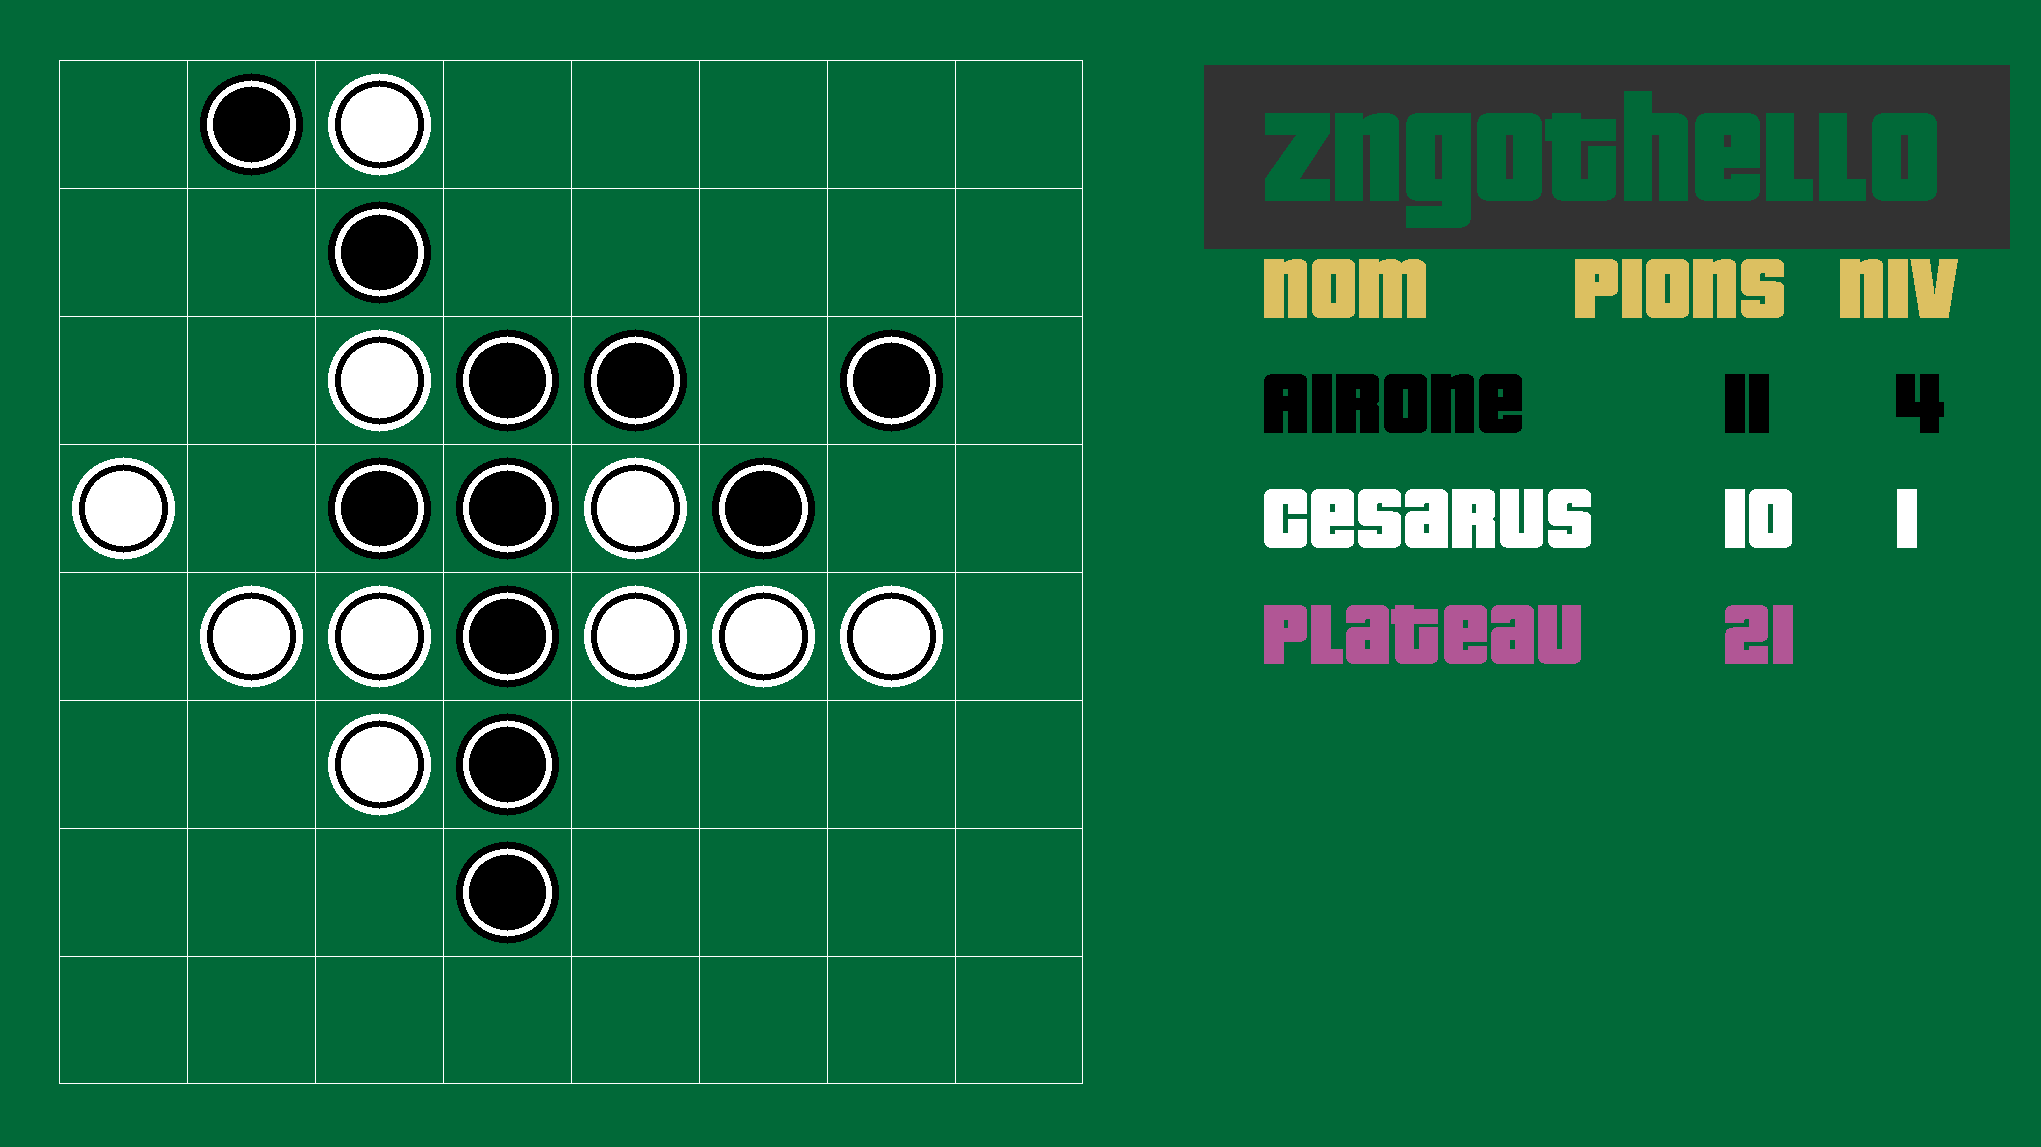
\includegraphics{zngOscreen.png} 
\end{center}
\caption{Stratégie gagnante}
\end{figure}

\newpage
\tableofcontents
\newpage

\section{Introduction}
  L'objectif de ce projet était de faire un premier pas vers la notion d'"Intelligence Artificielle" en codant le jeu de l'Othello. Dans ce rapport nous allons nous intéresser à l'I.A. de notre jeu, plus précisément à la façon dont nous l'avons codé et pourquoi de cette manière.
  

\section{Moyens utilisés}
\begin{itemize}
\item Machines avec distribution Ubuntu
\item Pour nous faciliter le travail de groupe : la plateforme github
\end{itemize}

\section{La fonction d'évaluation}
\begin{figure}
\begin{center}
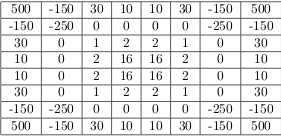
\includegraphics{tableothello.png} 
\end{center}
\caption{Stratégie gagnante}
\end{figure}

\section{Les niveaux de l'I.A.}
\subsection{Niveau 0}
Pour ce niveau il suffisait simplement de compléter une liste de coups possibles pour une couleur choisie, puis jouer un coup au hasard.
\subsection{Niveau 1, 2 et 3}
Pour ces trois niveaux qui reposaient sur le principe d'un parcours d'arbre de possibilités et de notation des fils avec la fonction d'évaluation. Nous avons décidé de ne pas utiliser de structure d'arbre n-aire (int **plateau, struct arbre **fils, int nbfils) pour une raison d'optimisation.
\newline
En effet, supposons qu'un plateau a n coups possibles, donc n fils puis que chaque fils a, par exemple, n+1 coups possibles. Nous devons donc stocker 1+n*(n+1) noeuds en mémoire et nous sommes à peine a une profondeur 1!
\newline
Pour remédier à ce problème nous avons pris la décision de faire de la façon suivante:
\begin{itemize}
\item Si nous avons pas encore atteint la profondeur souhaitée, copier le plateau (plateau\_bis) puis jouer un coup (pile de coup possibles) sur celui-ci. Rappeler la fonction avec plateau\_bis en paramètre et avec une profondeur de profondeur-1 tant que la pile de coups possibles n'est pas vide. Enfin libérer l'espace mémoire de plateau\_bis.
\item Si nous avons atteint la profondeur souhaitée, noter ce fils avec la fonction d'évaluation.
\end{itemize}
Donc avec l'algorithme minmax, c'est-à-dire pour les niveaux 1 et 2, il fallait regarder la note de tous les fils tandis qu'avec l'algorithme alpha-beta, pas besoin de parcourir tous les fils d'un noeud. Il est donc logique que le niveau 3 était plus réactif que le niveau 1 et 2 pour une même profondeur de parcours.
\subsection{Niveau 4}
Pour ce niveau, il s'agissait d'optimiser la gestion de la mémoire en utilisant qu'un seul plateau pour modéliser les coups possibles. Nous avons donc modéliser tous les coups possibles sur le même plateau de jeu que le joueur avec l'aide d'un pile de coups joués:
\begin{itemize}
\item À partir du plateau actuel, compléter la liste de coups possibles.
\item Jouer un coup de cette liste et l'empiler sur la pile de coups joués et le stocker
\item Répéter la même action (fonction récursive) jusqu'à avoir atteint la profondeur souhaitée et noter le plateau obtenue, stocker la note.
\item Enfin on dépile jusqu'à revenir au plateau initial.
\end{itemize}
En sortie du programme on obtient le coup le mieux noté.
\section{Conclusion}

\end{document}
